\documentclass{report}
\usepackage{amsfonts}
\usepackage{amsthm}
\usepackage{amsmath}
\usepackage{algorithmic}
\usepackage{algorithm}
\newtheorem{theorem}{Theorem}
\DeclareMathOperator{\diff}{diff}
\addtolength{\parskip}{3mm}
\title{\Huge\sc True Facts}
\author{Al Caveman}
\usepackage{graphicx}
\usepackage{eso-pic}
\newcommand\BackgroundPic{
\put(-5,-190){
\parbox[b][\paperheight]{\paperwidth}{%
\vfill
\centering
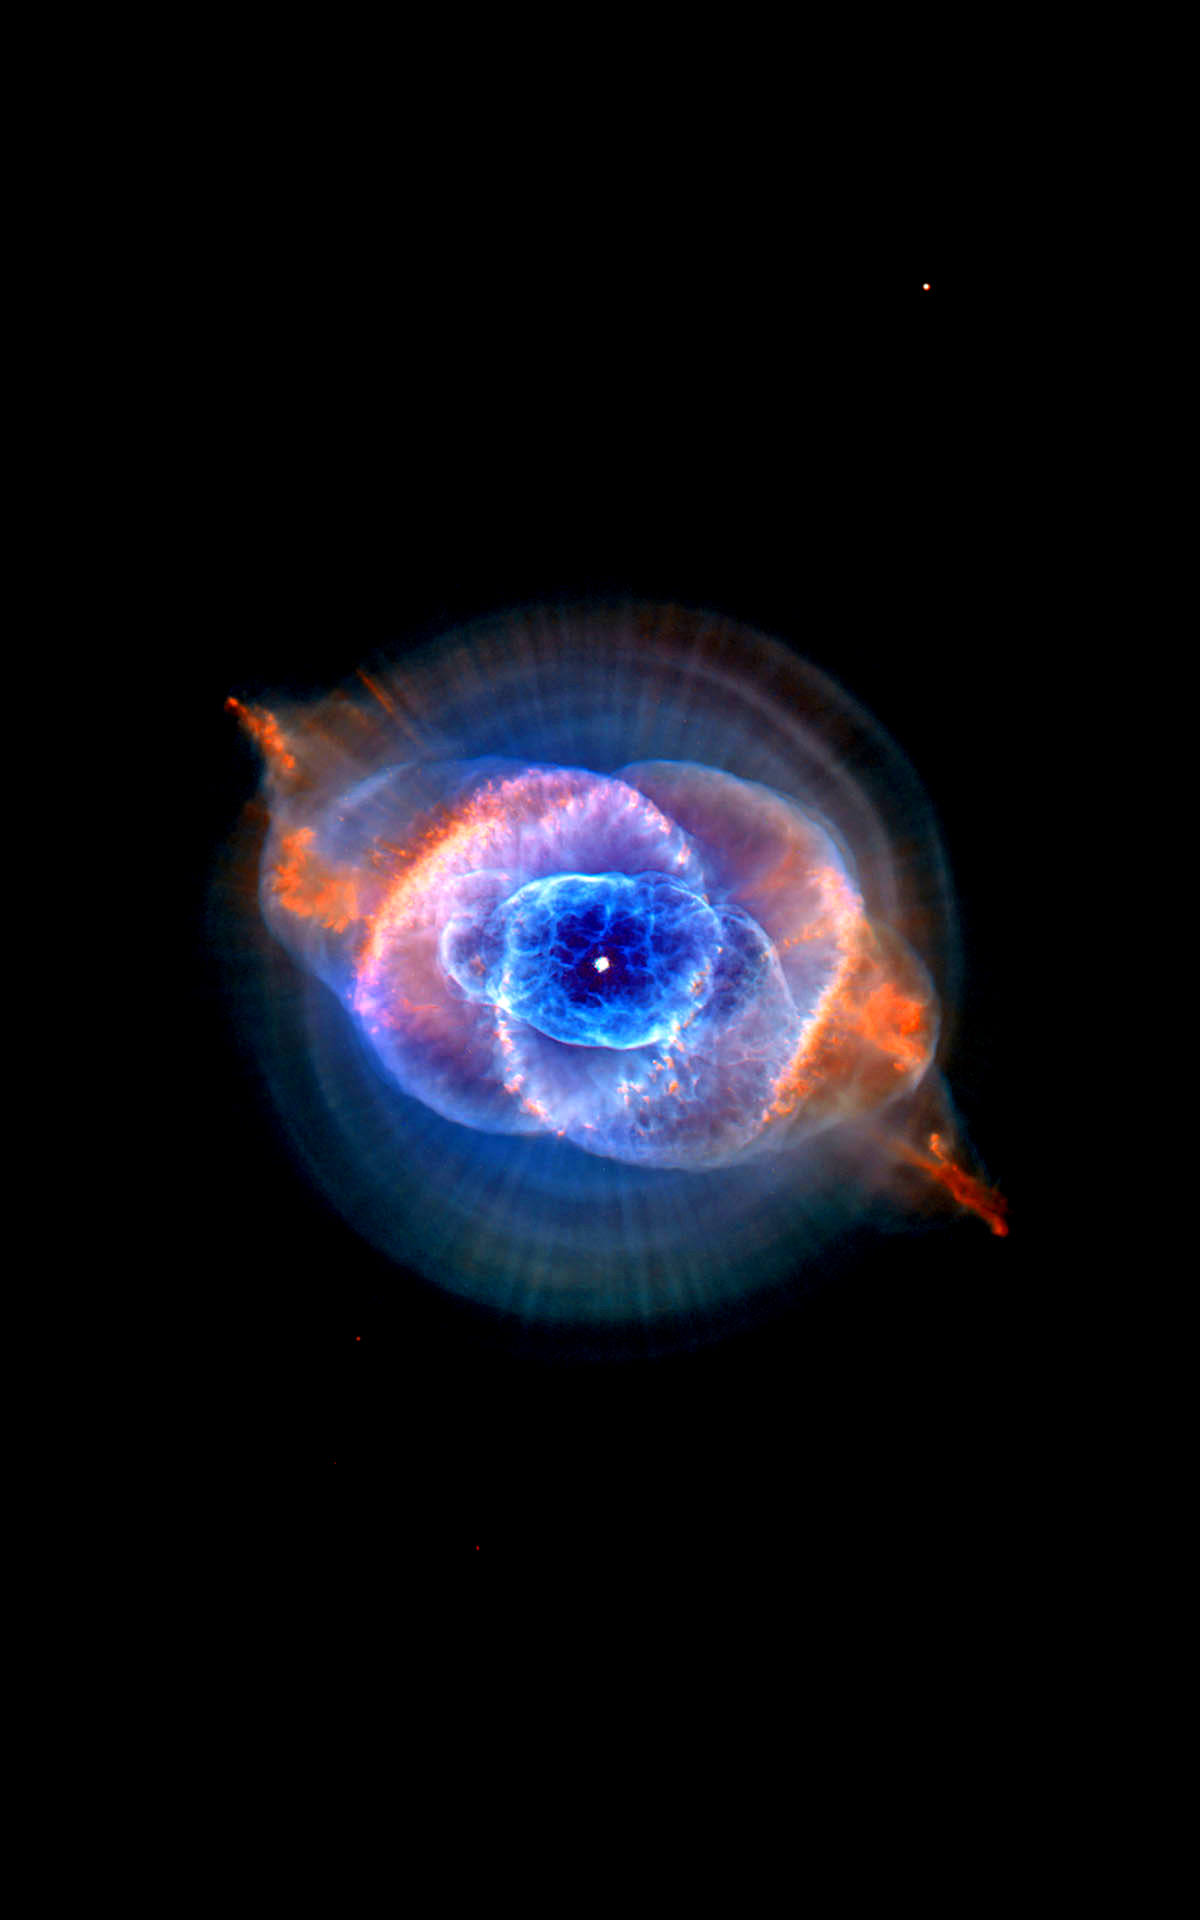
\includegraphics[width=1.01\paperwidth, keepaspectratio]{background.png}%
\vfill
}}}
\begin{document}
\AddToShipoutPicture*{\BackgroundPic}
\begin{titlepage}
\centering
\color{white}{{\Huge\sc True Facts}\\\vspace{1cm}\Large Al Caveman\\\vspace{0.5cm}2015}
\end{titlepage}

\chapter*{Preface}
This book's primary objective is to educate you about difficult/non-obvious
(but nonetheless important) facts about the universe that you live in. This
book is written with the spirit that you, monkeys, are able to learn.  This
book is also highly anticipated:
\begin{quote}
``\textbf{Al-Caveman:} RobbieAB$|$work, would u read my book?
\textbf{RobbieAB$|$work:} Depends how bored I am.
\textbf{Al-Caveman:} ok. i take that as \emph{yes}.'' ---
Freenode/\#gentoo-chat-exile, 2015
\end{quote}

\begin{quote}
``\textbf{Al-Caveman:} DistantStar, u?
\textbf{DistantStar:} okay. 
\textbf{Al-Caveman:} perfect.'' --- Freenode/\#gentoo-chat-exile, 2015
\end{quote}

\tableofcontents

\chapter{History}
You really must read this chapter. You can't just jump around to other sections
while expecting that you know what's goin on. Okay maybe you can, but if you
jump around then you are effectively most likely performing a less inefficient
use of your time than if you heed my advise.

\section{The Past}
Some say that the whole thing started by something that caused a big
explosion that resulted in lots of things some of which is making you exist.

Let's fast-forward and start from the point in time when monkeys started to
exist. Monkeys have been fucking each other for some time, and by doing so
they make more monkeys. Not all monkeys are alike.  Some monkeys live long
enough to fuck other monkeys, and some don't.

Turns out that the nature cares about only one thing: how well you survive.
Simply, the reason why things look like the way they are now, is because
this is the configuration that managed to keep existing.

There were some fascinating configurations, like the saber-toothed cat. But as
such wasn't able to survive and got extinct in a glimpse. The nature didn't
(and doesn't) give a damn rat's ass about how sexy the saber-toothed cats were
to the catesses of that era.

\section{The Present}
Currently, what we see is a continuation of evolution as you've seen in the
previous section on \emph{The Past}. The evolution is made of two parts: 1)
random mutations, and 2) natural-selection. This can be summarized into the
following randomized algorithm\footnote{Srsly DuckDuckGo randomized algorithms
if you don't know.}:

\begin{algorithm}
\caption{The algorithm that made you.}
\begin{algorithmic}
    \FOR{1 ... $t$}
    \IF{$x$ survives}
        \STATE{Keep it alive, and let it fuck around..}
    \ELSE
        \STATE{Let it die; i.e. make it into other things (conservatio law}
    \ENDIF
    \ENDFOR
\end{algorithmic}
\end{algorithm}

\begin{itemize}
    \item Randomly shuffles stuff (e.g. particles) around. This results in new
    permutations of the stuff. One of the permutations that exist now is
    \emph{you}. 
    \item Test if the created permutations can live. If they can live then let
    them live, and if they can't thive then let them not live. Easy peasy.
\end{itemize}

Basically, that is some kind of an algorithm that some smarty folks would like
to call a \emph{randomized algorithm}. One question is, what would happen in
the limit as time approaches infinity?

But before you go on, I assume that you know what is a randomized algorithm. If
you don't, then DuckDuckGo it and come back after educating yourself about it.


\section{The Future}
asfd




\chapter{Good and Bad}

\end{document}
